\section{Logical Design}

\subsection{Table of Volumes}

\begin{longtable}{|c|c|c|p{8cm}|}
    \hline
    \textbf{Concept} & \textbf{Concept Type} & \textbf{Volume} & \textbf{Why} \\
    \hline
    \endfirsthead
    \hline
    \textbf{Concept} & \textbf{Concept Type} & \textbf{Volume} & \textbf{Why} \\
    \hline
    \endhead
    Central Office & Entity & 1 & There is a single central office managing all operations \\
    \hline
    Divided & Relationship & 10 & Assuming each Central Office is divided into 10 Depots \\
    \hline
    Depot & Entity & 10 & Same as before \\
    \hline
    Operates & Relationship & 100 & By specifications each depot operates in 10 municipalities, then $10 \times 10 = 100$ \\
    \hline
    Municipality & Entity & 100 & Same as before \\
    \hline
    Composed & Relationship & 100 & Assuming each depot has on average 10 teams, then $10 \times 10 = 100$ \\
    \hline
    Team & Entity & 100 & By specifications there are 100 teams \\
    \hline
    Has & Relationship & 1000 & By specifications each team has on average 10 members, then $100 \times 10 = 1000$ \\
    \hline
    Member & Entity & 1000 & Same as before \\
    \hline
    Manages & Relationship & 5000 & Assuming each team handles on average 50 bookings, then $100 \times 50 = 5000$ \\
    \hline
    Booking & Entity & 5000 & Same as before \\
    \hline
    Recurrent Booking & Entity & 1000 & Assuming 20\% of bookings are recurrent, then $5000 \times 0.2 = 1000$ \\
    \hline
    One-time Booking & Entity & 4000 & Assuming 80\% of bookings are one-time, then $5000 \times 0.8 = 4000$ \\
    \hline
    Instance of & Relationship & 5000 & Each booking is an istance of only an installation \\
    \hline
    Installation & Entity & 50 & Assuming that each installation has on average 100 booking instances, then $5000 / 100 = 50$ \\
    \hline
    Promo & Entity & 10 & Assuming 20\% of installations are promotional, then $50 \times 0.2 = 10$ \\
    \hline
    Places & Relationship & 100 & Assuming each customer places on average 50 bookings, then $5000 / 50 = 100$ \\
    \hline
    Customer & Entity & 100 & Same as before \\
    \hline
    Individual & Entity & 50 & Assuming 50\% of customers are individuals, then $100 \times 0.5 = 50$ \\
    \hline
    Company & Entity & 50 & Assuming 50\% of customers are companies, then $100 \times 0.5 = 50$ \\
    \hline
    Organizes & Relationship & 1000 & Assuming each customer has on average 10 event locations, then $100 \times 10 = 1000$ \\
    \hline
    Event Location & Entity & 1000 & Same as before \\
    \hline
    Needs & Relationship & 5000 & Assuming each event location has on average 5 bookings, then $1000 \times 5 = 5000$ \\
    \hline
    \caption{Estimated volumes of conceptual entities}
    \label{tab:volumes-logical}
\end{longtable}

\subsection{Tables of Accesses}

\subsubsection{Operation \ref{op1}: Enter all data related to a new customer}

\begin{longtable}[H]{|c|c|c|c|p{7cm}|}
    \hline
    \textbf{Concept} & \textbf{Concept Type} & \textbf{Accesses} & \textbf{Acc. Type} & \textbf{Why} \\
    \hline
    \endfirsthead
    \hline
    \textbf{Concept} & \textbf{Concept Type} & \textbf{Accesses} & \textbf{Acc. Type} & \textbf{Why} \\
    \hline
    \endhead
    Customer & Entity & 1 & Write & Simply insert the new customer entity with their personal details and alphanumeric code \\
    \hline
    \caption{Accesses for Operation \ref{op1}}
    \label{tab:op1-accesses-logical}
\end{longtable}

\paragraph{Summary}
The total cost of Operation \ref{op1} is $1 \times 2 = 2$ units of cost (one write access), with a daily load cost of $2 \times 10 = 20$ units per day.

\subsubsection{Operation \ref{op2}: Record a new booking}

For this operation, we assume the following data is provided: customer ID, event location ID, team ID, and installation ID.

\begin{longtable}[H]{|p{2cm}|p{2cm}|p{1cm}|p{1cm}|p{7cm}|}
    \hline
    \textbf{Concept} & \textbf{Concept Type} & \textbf{Acc.} & \textbf{Acc. Type} & \textbf{Why} \\
    \hline
    \endfirsthead
    \hline
    \textbf{Concept} & \textbf{Concept Type} & \textbf{Accesses} & \textbf{Acc. Type} & \textbf{Why} \\
    \hline
    \endhead
    Booking & Entity & 1 & Write & Create a new booking entity with type, date, duration, and cost \\
    \hline
    Places & Relationship & 1 & Write & Establish the relationship between the booking and the customer (places) \\
    \hline
    Needs & Relationship & 1 & Write & Establish the relationship between the booking and the event location (needs) \\
    \hline
    Manages & Relationship & 1 & Write & Establish the relationship between the booking and the setup team (manages) \\
    \hline
    Instance of & Relationship & 1 & Write & Establish the relationship between the booking and the installation (instance of) \\
    \hline
    \caption{Accesses for Operation \ref{op2}}
    \label{tab:op2-accesses-logical}
\end{longtable}

If we consider also the redudancy of updating the number of installations made by the team and the setup time estimate for the event location, we would have the following additional accesses:

\begin{longtable}[H]{|p{2cm}|p{2cm}|p{1cm}|p{1cm}|p{7cm}|}
    \hline
    \textbf{Concept} & \textbf{Concept Type} & \textbf{Acc.} & \textbf{Acc. Type} & \textbf{Why} \\
    \hline
    Team & Entity & 1 & Read & Read the team entity to check its current installation count \\
    \hline
    Team & Entity & 1 & Write & Update the number of installations made by the team (increment by 1) \\
    \hline
\end{longtable}

If we also consider the redundancy of updating the setup time estimate for the event location, we would have the following additional accesses:

\begin{longtable}[H]{|p{2cm}|p{2cm}|p{1cm}|p{1cm}|p{7cm}|}
    \hline
    \textbf{Concept} & \textbf{Concept Type} & \textbf{Acc.} & \textbf{Acc. Type} & \textbf{Why} \\
    \hline
    Event Location & Entity & 1 & Read & Read the event location entity to check its current setup time estimate \\
    \hline
    Event Location & Entity & 1 & Write & Update the setup time estimate for the event location (increment by the setup time of the installation) \\
    \hline
\end{longtable}

\paragraph{Summary}
The total cost of Operation \ref{op2} is $5 \times 2 = 10$ units of cost (five write accesses), with a daily load cost of $10 \times 300 = 3000$ units per day. If we consider also the redundancy of updating the number of installations made by the team, the total cost would be $6 \times 2 + 1 = 13$ units of cost (seven write accesses), with a daily load cost of $13 \times 300 = 3900$ units per day. If we also consider the redundancy of updating the setup time estimate for the event location, the total cost would be $6 \times 2 + 1 = 13$ units of cost (nine write accesses), with a daily load cost of $13 \times 300 = 3900$ units per day. If we consider both redundancies together, the total cost would be $7 \times 2 + 2 = 16$ units of cost (eleven write accesses), with a daily load cost of $16 \times 300 = 4800$ units per day.

\subsubsection{Operation \ref{op3}: Register a new event location}

For this operation, we assume the customer ID is provided as input.

\begin{longtable}[H]{|p{2cm}|p{2cm}|p{2cm}|p{2cm}|p{7cm}|}
    \hline
    \textbf{Concept} & \textbf{Concept Type} & \textbf{Acc.} & \textbf{Acc. Type} & \textbf{Why} \\
    \hline
    \endfirsthead
    \hline
    \textbf{Concept} & \textbf{Concept Type} & \textbf{Accesses} & \textbf{Acc. Type} & \textbf{Why} \\
    \hline
    \endhead
    Event Location & Entity & 1 & Write & Create a new event location entity with address, postal code, city, province, setup time estimate, and equipment capacity \\
    \hline
    Organizes & Relationship & 1 & Write & Establish the relationship between the event location and the customer (organizes) \\
    \hline
    \caption{Accesses for Operation \ref{op3}}
    \label{tab:op3-accesses-logical}
\end{longtable}

\paragraph{Summary}
The total cost of Operation \ref{op3} is $2 \times 2 = 4$ units of cost (two write accesses), with a daily load cost of $4 \times 50 = 200$ units per day.

\subsubsection{Operation \ref{op4}: View the team that handled setups at a specific event location}

For this operation, we assume the event location ID is provided as input.

\begin{longtable}[H]{|p{2cm}|p{2cm}|p{2cm}|p{2cm}|p{7cm}|}
    \hline
    \textbf{Concept} & \textbf{Concept Type} & \textbf{Accesses} & \textbf{Acc. Type} & \textbf{Why} \\
    \hline
    \endfirsthead
    \hline
    \textbf{Concept} & \textbf{Concept Type} & \textbf{Accesses} & \textbf{Acc. Type} & \textbf{Why} \\
    \hline
    \endhead
    Event Location & Entity & 1 & Read & Access the event location to identify its associated bookings \\
    \hline
    Needs & Relationship & 5 & Read & Navigate the needs relationship to retrieve the bookings associated with the event location (assuming on average 5 bookings per event location) \\
    \hline
    Booking & Entity & 5 & Read & On average, read 5 booking entities related to the event location \\
    \hline
    Manages & Relationship & 5 & Read & Navigate the manages relationship to retrieve the setup teams associated with each booking \\
    \hline
    Setup Team & Entity & 5 & Read & Retrieve the setup team entities that handled the setups \\
    \hline
    \caption{Accesses for Operation \ref{op4}}
    \label{tab:op4-accesses-logical}
\end{longtable}

\paragraph{Summary}
The total cost of Operation \ref{op4} is $21 \times 1 = 21$ units of cost (twenty-one read accesses), with a daily load cost of $21 \times 20 = 420$ units per day.

\subsubsection{Operation \ref{op5}: Print a list of event locations sorted by number of bookings}

\begin{longtable}[H]{|p{2cm}|p{2cm}|p{2cm}|p{2cm}|p{7cm}|}
    \hline
    \textbf{Concept} & \textbf{Concept Type} & \textbf{Accesses} & \textbf{Acc. Type} & \textbf{Why} \\
    \hline
    \endfirsthead
    \hline
    \textbf{Concept} & \textbf{Concept Type} & \textbf{Accesses} & \textbf{Acc. Type} & \textbf{Why} \\
    \hline
    \endhead
    Event Location & Entity & 1000 & Read & Read all event location entities to retrieve their information \\
    \hline
    % Booking & Entity & 5000 & Read & Read all booking entities to count the number of bookings per event location \\
    % \hline
    Needs & Relationship & 5000 & Read & Navigate the needs relationship to associate bookings with event locations for counting \\
    \hline
    \caption{Accesses for Operation \ref{op5}}
    \label{tab:op5-accesses-logical}
\end{longtable}

\paragraph{Summary}
The total cost of Operation \ref{op5} is $6000 \times 1 = 6000$ units of cost (six thousand read accesses), with a daily load cost of $6000 \times 5 = 30000$ units per day.

\subsection{ER Schema Refactoring}

\paragraph{Generalization/Specialization Analysis}

Individual and Company specializations of the Customer entity will hold different attributes so it is not possible to merge them together. Also the Recurring specialization of the Booking entity will hold different attributes compared to the One-time specialization so it is not possible to merge them together. Finally also the Promo specialization of the Installation entity will hold different attributes compared to the regular Installation entity so it is not possible to merge them together. Therefore, we keep the current structure of the schema with all of its generalizations or specializations.

\paragraph{Redudancies Analysis}

A first redudancy is the places relationship between Customer and Booking, which can be inferred from the organizes relationship between Customer and Event Location and the needs relationship between Event Location and Booking. Since adding this relationship would require a trigger to check that the customer placing the booking is the same as the one organizing the event location (with a non ignorable overhead), and this information can be easily inferred from the existing relationships, we decided to remove the places relationship from the schema. This decision is also supported by the fact that there are no common or frequent operations defined in the use case requirements that would require direct access to this relationship, so we can afford to infer this information when needed without incurring in significant performance issues.

The second redundancy we can identify is the number of installations made by each team, which can be calculated as the count of bookings handled by that team. Instead of storing this information as an attribute of the Team entity, we can calculate it on the fly when needed, using a query that counts the number of bookings associated with each team through the manages relationship. This would eliminate the need for redundant updates to this attribute whenever a new booking is recorded. However, since the cost of keeping this attribute updated is not significant (just one additional write access per new booking), and we could expect in the future to frequently access the number of installations made by each team, we decided to keep this attribute in the Team entity and update it whenever a new booking is recorded, accepting the redundancy for the sake of faster reads.

The third redundancy we can identify is the setup time estimate for each event location, which can be calculated as the sum of the setup times of all bookings handled at that location. Similar to the previous case, we can choose to calculate this information on the fly when needed, using a query that sums the setup times of bookings associated with each event location through the needs relationship. This would eliminate the need for redundant updates to this attribute whenever a new booking is recorded. However, also in this case the cost of keeping this attribute updated is not significant (just one additional write access per new booking), and we could expect that a customer will frequently access the setup time estimate for each event location, we decided to keep this attribute in the Event Location entity and update it whenever a new booking is recorded, accepting the redundancy for the sake of faster reads.

The fourth and fifth redudancies involve the number of employees in each depot and central office, which can be calculated as the sum of the members of all teams in that depot or central office respectively. Similar to the previous cases, we can choose to calculate this information on the fly when needed, using queries that sum the number of members of teams associated with each depot or central office through the composed relationship. This would eliminate the need for redundant updates to these attributes whenever a new team member is added or removed. 

However computing such an aggregate query on the fly might be too costly in terms of performance, especially if we have a large number of teams and members. Additionally, there are no common or frequent update operations on teams, depots and central offices defined in the use case requirements that would justify the need to remove these attributes from the schema. Since updates on these involved entities are not common and we want to optimize for read performance (on those cases), we decided to keep these attributes in the Depot and Central Office entities and update them whenever a new team member is added or removed, accepting the redundancy for the sake of faster reads.

\paragraph{Partioning and Merging of Entities/Relationships}

Given the current schema, there are no candidates for partitioning or merging entities or relationships. The entities and relationships are well-defined and do not exhibit significant overlap or redundancy that would suggest a need for merging. Additionally, the entities and relationships are not large or complex enough to warrant partitioning for performance and semantical reasons. Therefore, we can keep the current structure of the schema without any partitioning or merging.

\paragraph{Primary Identifiers Design}

In order to correctly identify event locations and bookings, we added a unique numeric code automatically generated as a primary key for each new event location and booking. This will be implemented, in Oracle, using sequences that will generate a new unique value for each new record inserted into the Event Location and Booking tables. For depots, central offices and installations we choosed to use the name as primary key since it is a unique identifier for these entities and it is not expected to change over time.

\subsection{Logical Schema}

% add the logical-schema.png image here
\begin{figure}[H]
    \centering
    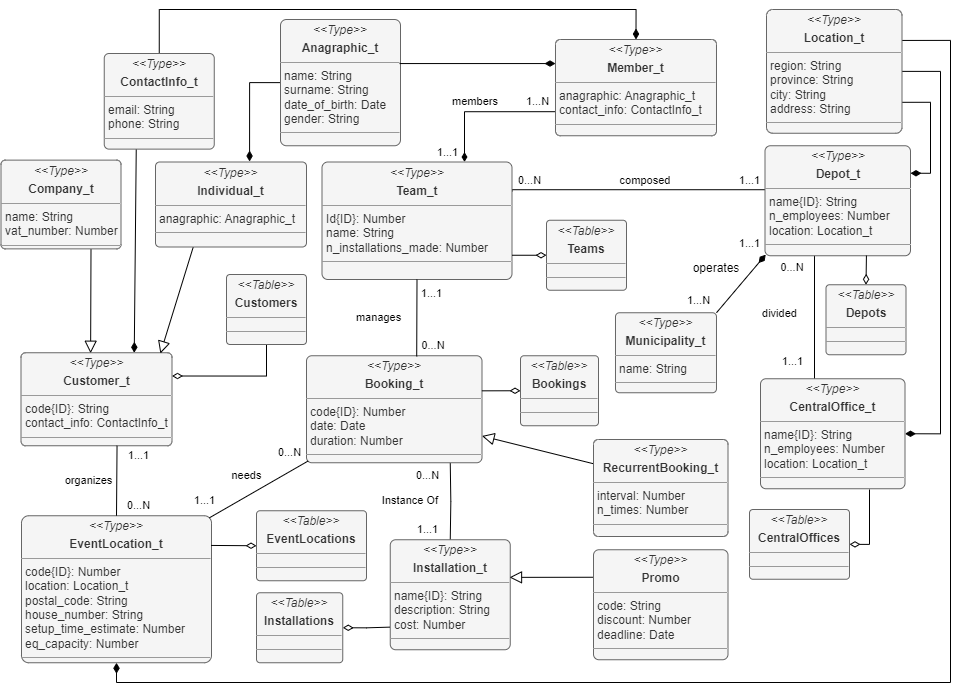
\includegraphics[width=1\textwidth]{./rsc/logical-schema.png}
    \caption{Logical Schema}
    \label{fig:logical-schema}
\end{figure}


